\documentclass[]{beamer}
% Class options include: notes, notesonly, handout, trans,
%                        hidesubsections, shadesubsections,
%                        inrow, blue, red, grey, brown

% Theme for beamer presentation.
\usepackage{beamerthemesplit} 



%%%%%%%%%%%%%%%%%%%%%%%%%%%%%%%%%%%%%%%%%%%%%%%%%%%%%%%%%%%%%%%%%%%%%%



\definecolor{mypink1}{rgb}{0.858, 0.188, 0.478}

\newcommand{\mybox}{%
    \collectbox{%
        \setlength{\fboxsep}{1pt}%
        \fbox{\BOXCONTENT}%
    }%
}

%%%%%%%%%%%%%%%%%%%%%%%%%%%%%%%%%%%%%%%%%%%%%%%%%%%%%%%%%%%%%%%%%%%%%%
% Other themes include: beamerthemebars, beamerthemelined, 
%                       beamerthemetree, beamerthemetreebars  

\title{PHY250: Waves 2D}    % Enter your title between curly braces
\author{Anabela R. Turlione}                 % Enter your name between curly braces
\institute{Digipen}      % Enter your institute name between curly braces
\date{Fall 2021}                    % Enter the date or \today between curly braces


\begin{document}

% Creates title page of slide show using above information
\begin{frame}
  \titlepage
\end{frame}
%\note{Talk for 30 minutes} % Add notes to yourself that will be displayed when
                           % typeset with the notes or notesonly class options

\section[]{}

% Creates table of contents slide incorporating
% all \section and \subsection commands
\begin{frame}
  \tableofcontents
\end{frame}


% \begin{frame}
%   % \centering
%    \movie[externalviewer]{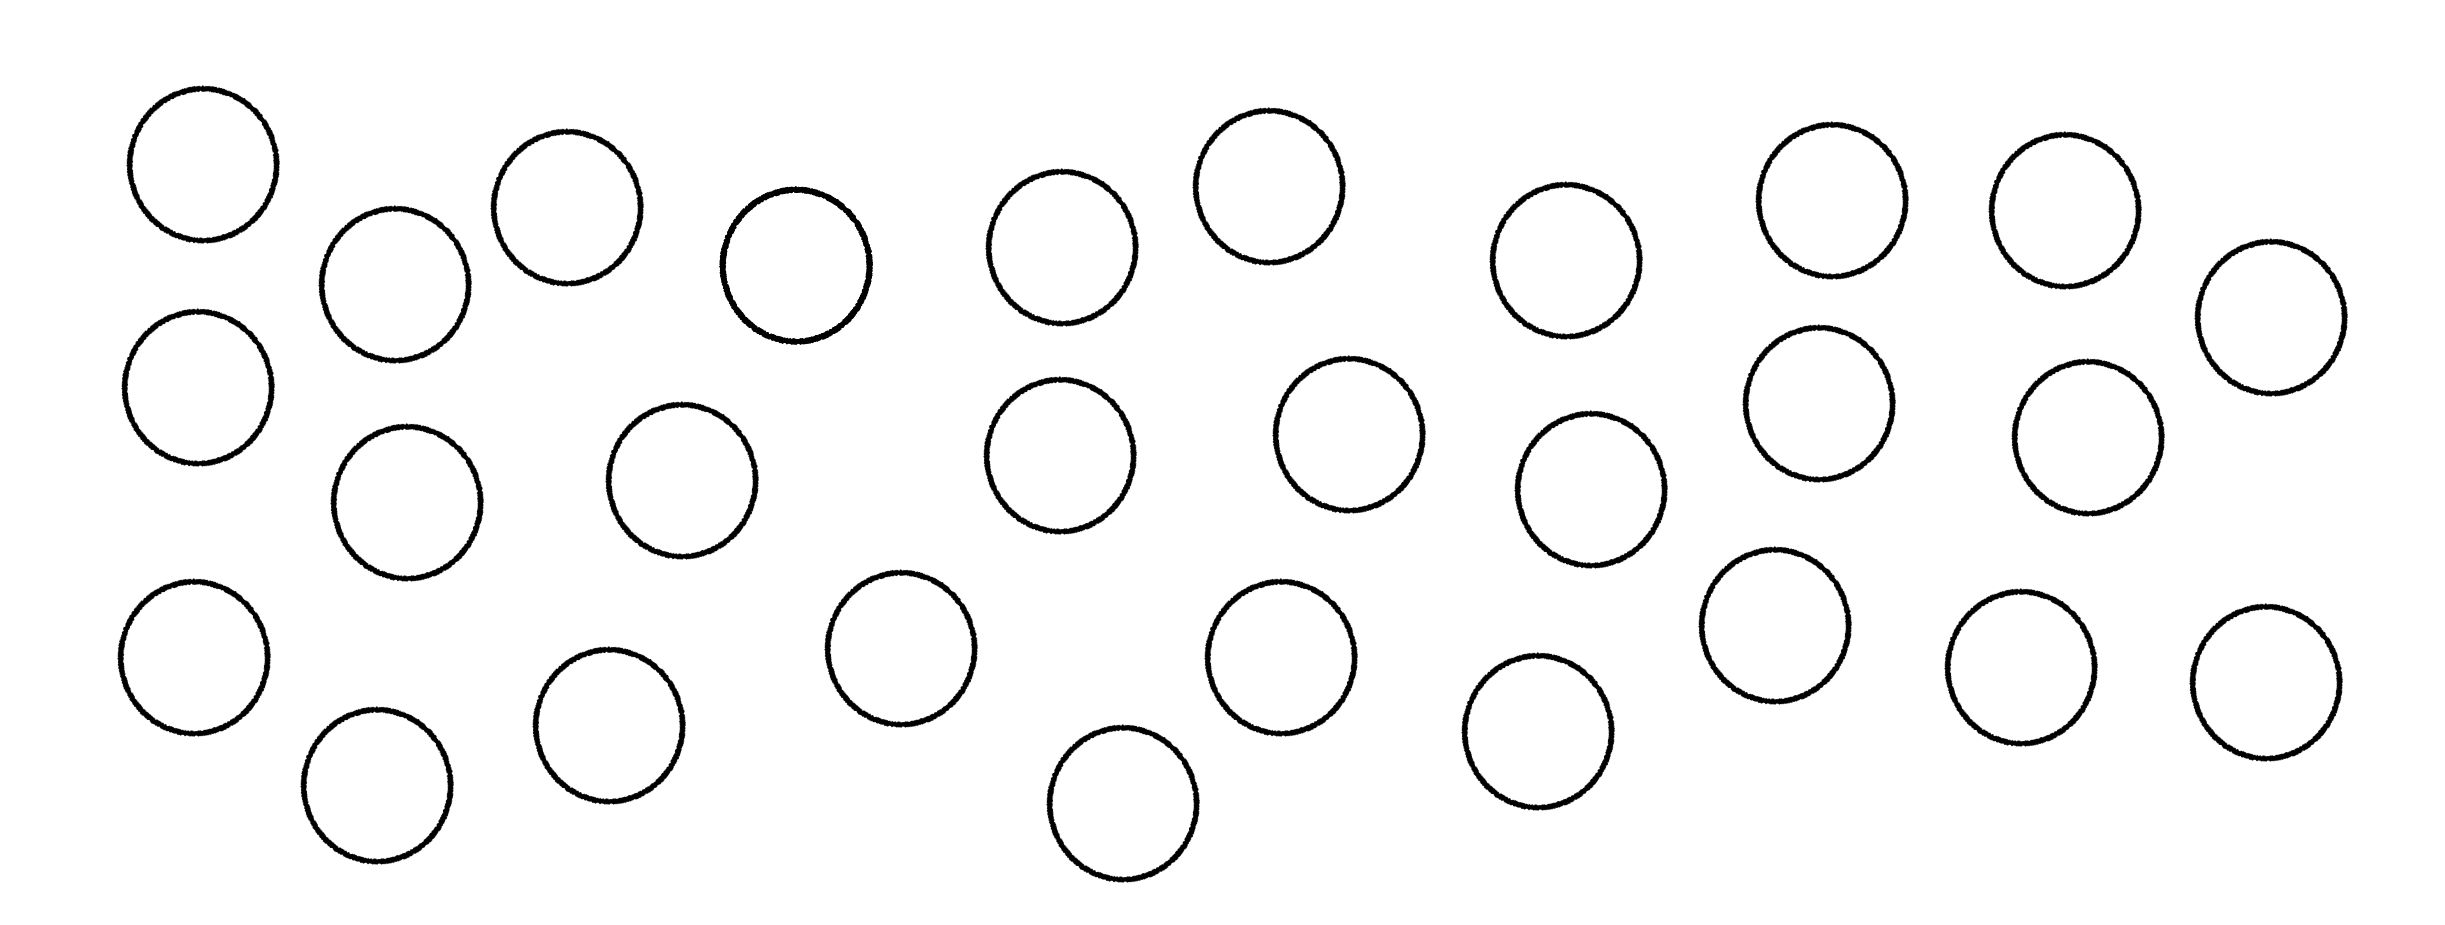
\includegraphics[width=\textheight ,
%    keepaspectratio]{surfacet1.jpg}}{test.mp4}

% \end{frame}
%%%%%%%%%%%%%%%%%%%%%%%%%%%%%%%%%%%%%%%%%%%%%%%%%%%%%%%%%%%%%%%%%%%

%%%%%%%%%%%%%%%%%%%%%%%%%%%%%%%%%%%%%%%%%%%%%%%%%%%%%%%%%%%%%%%%%%%


%%%%%%%%%%%%%%%%%%%%%%%%%%%%%%%%%%%%%%%%%%%%%%%%%




    
    
    
  

%%%%%%%%%%%%%%%%%%%%%%%%%%%%%%%%%%%%%%%%%%%%%%%%%%%%%%%%%%%%%%%

\section{Waves in 2D}

%%%%%%%%%%%%%%%%%%%%%%%%%%%%%%%%%%%%%%%%%%%%%%%%%%%%%%%%%%%%%%%
\subsection{Waves equation}

\begin{frame}
  \frametitle{Wave Equation }
  

  \begin{equation*}
    \frac{\partial^2 }{\partial t^2} D(t,x,y) =v^2\bigg[ \frac{\partial^2}{\partial x^2} D(t,x,y)+\frac{\partial^2 }{\partial y^2}D(t,x,y)\bigg]
  \end{equation*}
  
\vspace{5mm}


  \pause
Assumptions
\pause
\vspace{3mm}

  \begin{itemize}
    \item Uniform density.\pause
    \item Uniform tension.\pause
    \item Small oscillations.\pause
  \end{itemize}



  

    \end{frame}
  
  
  %%%%%%%%%%%%%%%%%%%%%%%%%%%%%%%%%%%%%%%%%%%%%%%%%%%%%%%%%%%%%%%


\begin{frame}
  \frametitle{Solutions}
  
Traveling waves:

\begin{equation*}
  D(t,\vec{r})=Asin(\vec{k}\cdot \vec{r}-\omega t)
\end{equation*}

  \begin{figure}[h!]
    \begin{center}
      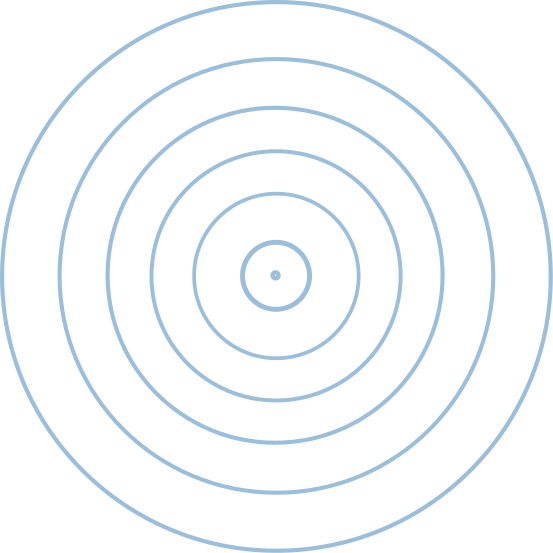
\includegraphics[height=2.in]{images4/top_view.png}
    \end{center}
  \end{figure}
  

  

    \end{frame}
  
  %%%%%%%%%%%%%%%%%%%%%%%%%%%%%%%%%%%%%%%%%%%%%%%%%%%%%%%%%%%%%%%



\begin{frame}
  \frametitle{Solutions}
  
Standing waves:

\begin{equation*}
  D(t,\vec{r})=A_{nm}sin(\frac{n\pi x}{L_x})sin(\frac{m\pi y}{L_y})cos(\omega t)
\end{equation*}

  \begin{figure}[h!]
    \begin{center}
      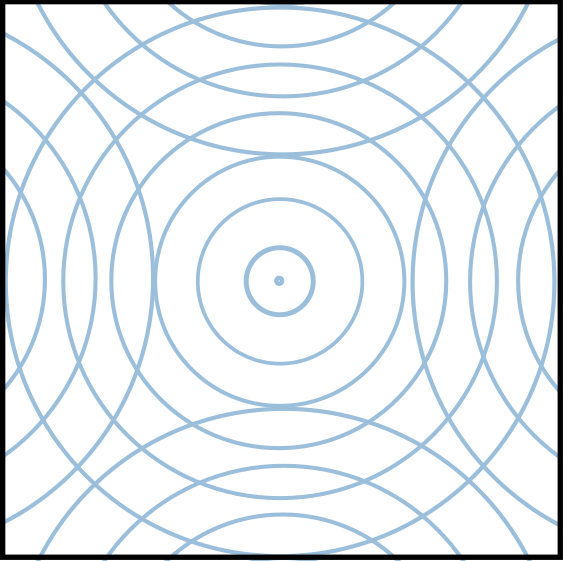
\includegraphics[height=2.in]{images4/top_view2.png}
    \end{center}
  \end{figure}
  

  

    \end{frame}

    
    %%%%%%%%%%%%%%%%%%%%%%%%%%%%%%%%%%%%%%%%%%%%%%%%%%%%%%%%%%%%%%%
  
  
    \begin{frame}
      \frametitle{Fourier in 2D }
      Combination of Harmonics
      \begin{equation*}
        D(t,\vec{r})=\sum_m\sum_n  A_{nm}sin(\frac{n\pi x}{L_x})sin(\frac{m\pi y}{L_y})cos(\omega t)
      \end{equation*}
      
      

    
      \end{frame}



%%%%%%%%%%%%%%%%%%%%%%%%%%%%%%%%%%%%%%%%%%%%%%%%%%%%%%%%%%%%%%%


\begin{frame}
  \frametitle{Waves in 2D  }
  
  
  
  
  For a two- or three-dimensional wave, such as a water wave, we are concerned
  with wave fronts, by which we mean all the points along the wave forming the
  wave crest.
  
  
  
    \begin{center}
    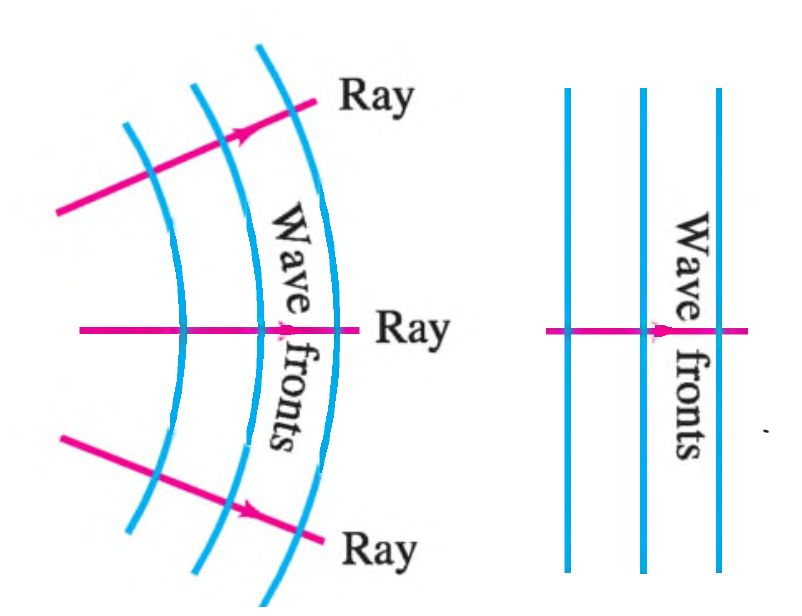
\includegraphics[height=1.7in]{images4/13.jpg}
  \end{center}
  
    \end{frame}
  
  
  
  %%%%%%%%%%%%%%%%%%%%%%%%%%%%%%%%%%%%%%%%%%%%%%%%%%%%%%%%%%%%%%%
  
  
  \begin{frame}
  \frametitle{Waves in 2D }
  
  
  
  
  
  
  A line drawn in the direction of motion, perpendicular to the wave front, is called a ray.
  
  
  
    \begin{center}
    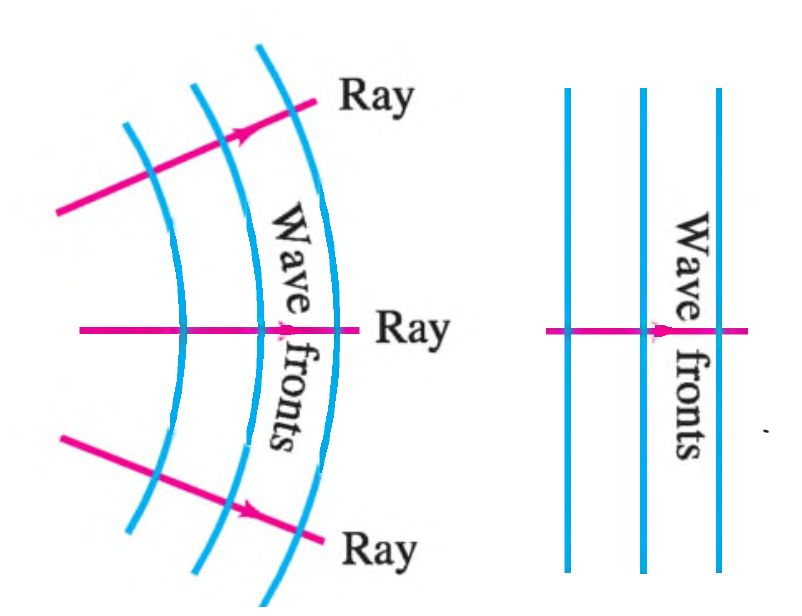
\includegraphics[height=1.7in]{images4/13.jpg}
  \end{center}
  
    \end{frame}
  
  
  
  %%%%%%%%%%%%%%%%%%%%%%%%%%%%%%%%%%%%%%%%%%%%%%%%%%%%%%%%%%%%%%%
  
  
  \begin{frame}
  \frametitle{Waves in 2D }
  
  
  
  
  Wave fronts far from the source have lost almost all their
  curvature  and are nearly straight; they are
  then called plane waves.
  
  
    \begin{center}
    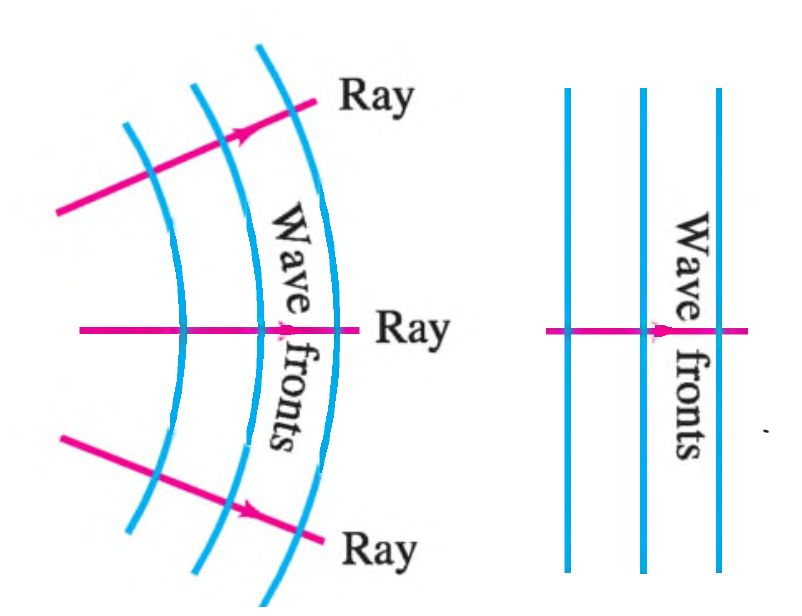
\includegraphics[height=1.7in]{images4/13.jpg}
  \end{center}
  
    \end{frame}



%%%%%%%%%%%%%%%%%%%%%%%%%%%%%%%%%%%%%%%%%%%%%%%%%%%%%%%%%%%%%%%


%%%%%%%%%%%%%%%%%%%%%%%%%%%%%%%%%%%%%%%%%%%%%%%%%%%%%%%%%%%%%%%


\begin{frame}
  \frametitle{Reflection and transmission }
  
  
  
  
  For a two- or three-dimensional wave, such as a water wave, we are concerned
  with wave fronts, by which we mean all the points along the wave forming the
  wave crest.
  
  
  
    \begin{center}
    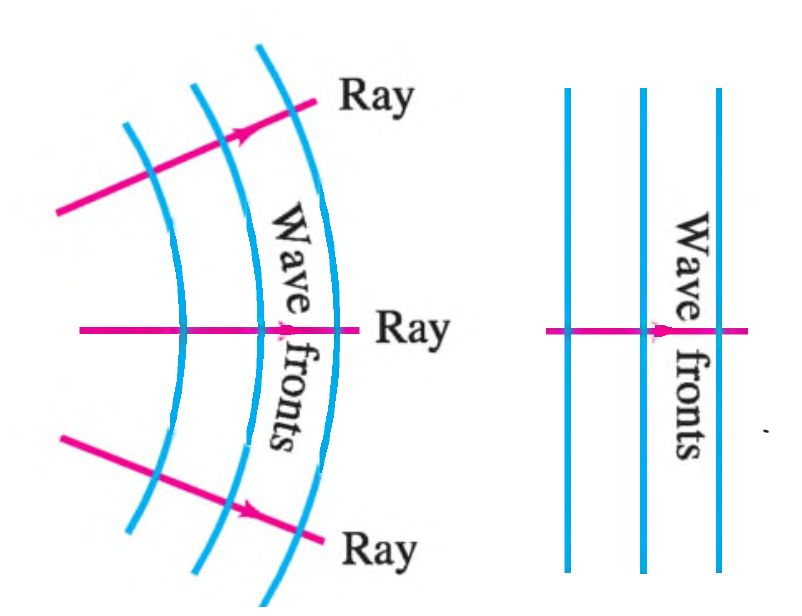
\includegraphics[height=1.7in]{images4/13.jpg}
  \end{center}
  
    \end{frame}
  
  
  
  %%%%%%%%%%%%%%%%%%%%%%%%%%%%%%%%%%%%%%%%%%%%%%%%%%%%%%%%%%%%%%%
  
  
  \begin{frame}
  \frametitle{Reflection and transmission }
  
  
  
  
  
  
  A line drawn in the direction of motion, perpendicular to the wave front, is called a ray.
  
  
  
    \begin{center}
    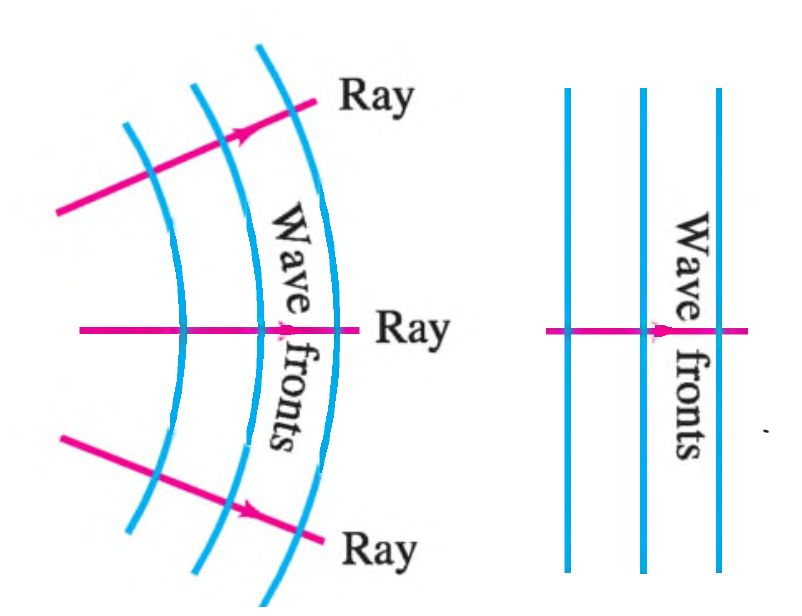
\includegraphics[height=1.7in]{images4/13.jpg}
  \end{center}
  
    \end{frame}
  
  
  
  %%%%%%%%%%%%%%%%%%%%%%%%%%%%%%%%%%%%%%%%%%%%%%%%%%%%%%%%%%%%%%%
  
  
  \begin{frame}
  \frametitle{Reflection and transmission }
  
  
  
  
  Wave fronts far from the source have lost almost all their
  curvature  and are nearly straight; they are
  then called plane waves.
  
  
    \begin{center}
    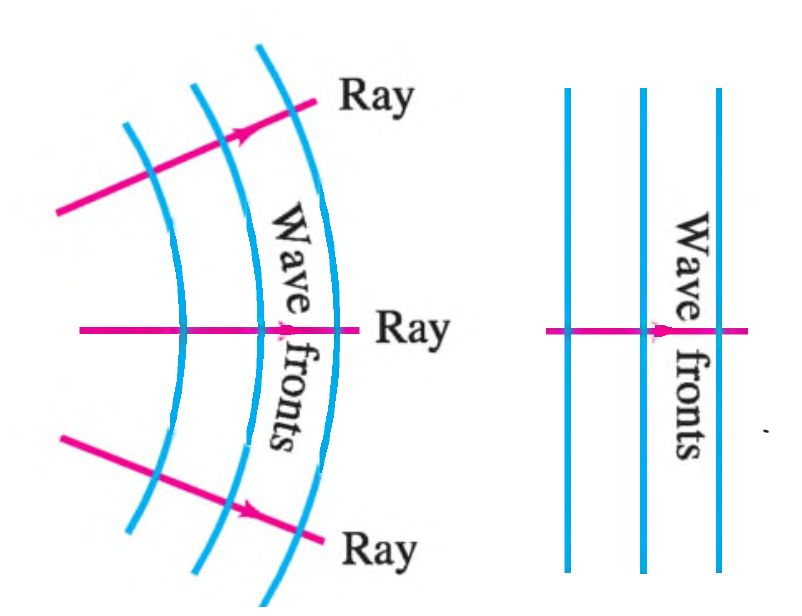
\includegraphics[height=1.7in]{images4/13.jpg}
  \end{center}
  
    \end{frame}

\begin{frame}
\frametitle{Interference }

Two sources sending identical waves in a medium. \pause Example two rocks thrown simultaneously in water: 




  \begin{center}
  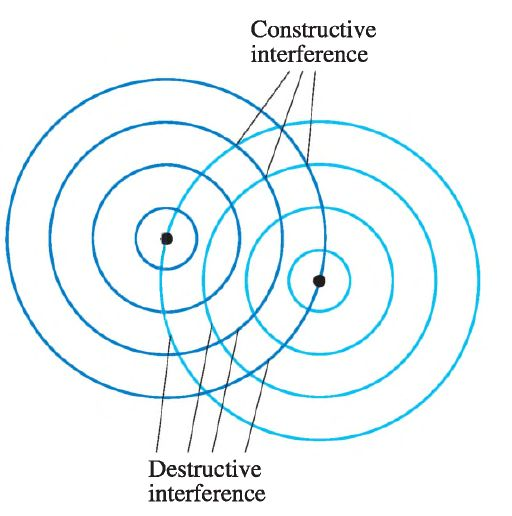
\includegraphics[height=2.3in]{images4/16.jpg}
\end{center}



  \end{frame}




%%%%%%%%%%%%%%%%%%%%%%%%%%%%%%%%%%%%%%%%%%%%%%%%%%%%%%%%%%%%%%%%%%%%%%%%%%%%%%%%%%%%%%%%%%%%%%%%%
\begin{frame}
  \frametitle{Spatial interference}
  
  When two waves, with the same frequency, simultaneously pass through the
  same region of space, they interfere with one another. Interference also occurs
  with sound waves.
  
  
  
    \begin{columns}[c]
     \column{2in}  % slides are 3in high by 5in wide
    
  
    \begin{center}
    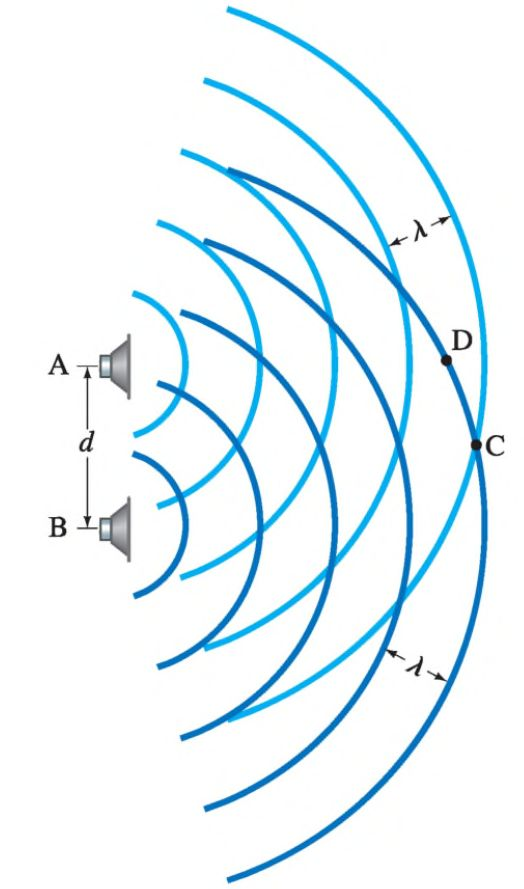
\includegraphics[height=1.8in]{images4/soundinterference.jpg}
  \end{center}
  
  
     \column{2in}
  
  \begin{itemize}
  \item  Point C (same distance from each speaker) $\pause \rightarrow$ loud sound ( constructive interference).
  \pause 
  
  \item Point  D, no sound or  little sound  (destructive interference).
  \end{itemize}
  
  
     \end{columns}
    \end{frame}
  
  
  
\begin{frame}%%%%%%%%%%%%%%%%%%%%%%%%%%%%%%%%%%%%%%%%%%%
\frametitle{Spacial interference}


  \begin{columns}[c]
   \column{2in}  % slides are 3in high by 5in wide
  
  \begin{center}
  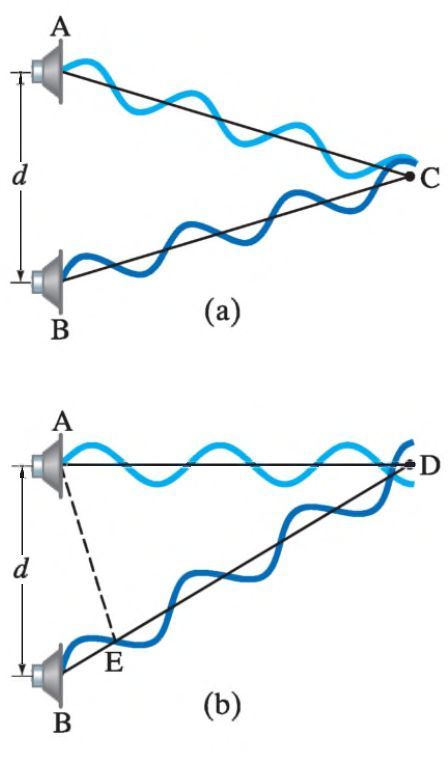
\includegraphics[height=2.in]{images4/soundinterference2.jpg}
\end{center}


   \column{2in}
\pause

  $ED=AD$,  If  $BE=\lambda/2$  the two waves will be exactly out of
phase when they reach D
\pause
\vspace{3mm}

 $\rightarrow$ destructive interference.

\pause
Then..

\begin{itemize}
\item $BD-AD=2\lambda, 3\lambda,...\rightarrow$ constructive interference
\pause

\item $BD-AD=\lambda/2, 3\lambda/2, 5\lambda/2,...\rightarrow$ destructive interference
\end{itemize}


   \end{columns}
  \end{frame}

%%%%%%%%%%%%%%%%%%%%%%%%%%%%%%%%%%%%%%%%%%%%%%%%%%%%%%%%%%%%%%%

% \begin{frame}
% \frametitle{Example}

% Two loudspeakers are $1.00~m$
% apart. A person stands $4.00~m$ from one speaker. How far must this person must be
% from the second speaker to detect destructive interference when the speakers
% emit an 1150-Hz sound? Assume the temperature is 20°C.

%   \end{frame}




%%%%%%%%%%%%%%%%%%%%%%%%%%%%%%%%%%%%%%%%%%%%%%%%%%%%%%%%%%%%%%%
\subsection{Doppler Effect}

\begin{frame}
\frametitle{Doppler Effect}

Change in Pitch when a source of sound is moving toward or moving away from the observer. 




  \end{frame}




%%%%%%%%%%%%%%%%%%%%%%%%%%%%%%%%%%%%%%%%%%%%%%%%%%%%%%%%%%%%%%%

\begin{frame}
\frametitle{Doppler Effect}




\begin{columns}[c]
  \column{2in}  % slides are 3in high by 5in wide

  \begin{center}
    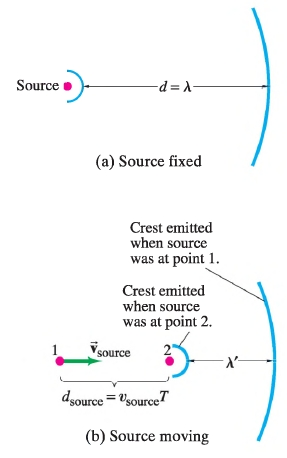
\includegraphics[height=2.8in]{images4/doppler1_b.jpg}
  \end{center} 
  \column{2in}

  Source at rest $\pause\rightarrow$ the wave travels at the velocity of sound in the air.
  \pause
  
  \vspace{3mm}

  Its velocity is independent of the source velocity.





  \end{columns}



  \end{frame}





%%%%%%%%%%%%%%%%%%%%%%%%%%%%%%%%%%%%%%%%%%%%%%%%%%%%%%%%%%%%%%%

% \begin{frame}
% \frametitle{Doppler Effect}

% Change in Pitch when a source of sound is moving toward or moving away from the observer. 

% \vspace{3mm}

% Source at rest $\rightarrow$ the wave travels at the velocity of sound in the air.



%   \begin{center}
%   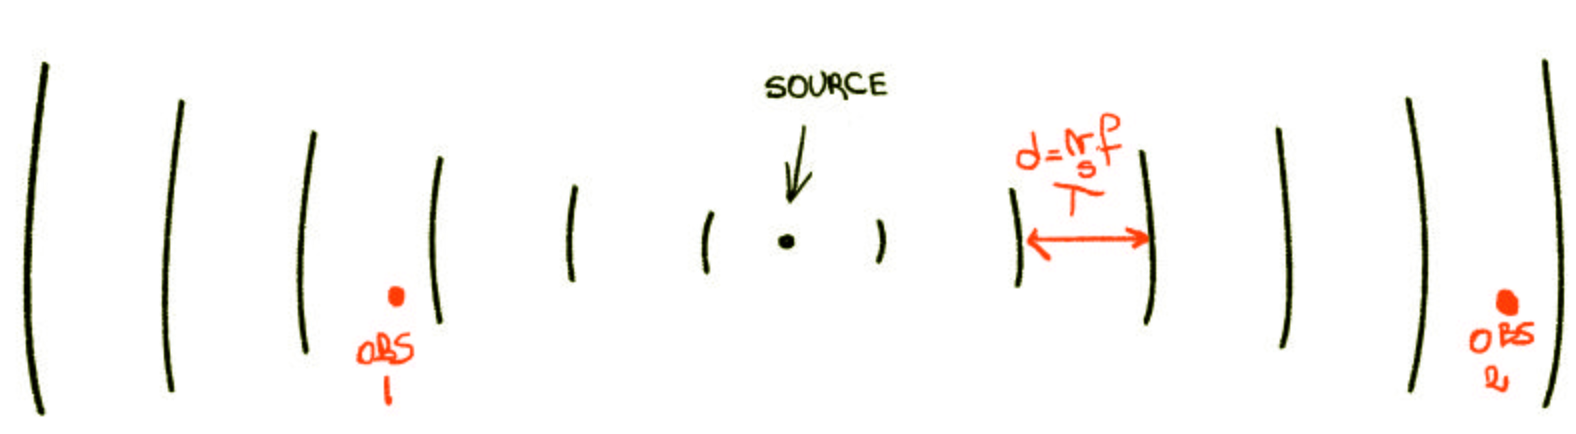
\includegraphics[height=1.2in]{images4/doppler2.jpg}
% \end{center}


%   \end{frame}






%%%%%%%%%%%%%%%%%%%%%%%%%%%%%%%%%%%%%%%%%%%%%%%%%%%%%%%%%%%%%%%
% \begin{frame}
% \frametitle{Doppler Effect}



% Source in motion $\rightarrow$ the wave travels at the velocity of sound in the air (its velocity is independent of the source velocity).

% \pause


%   \begin{center}
%   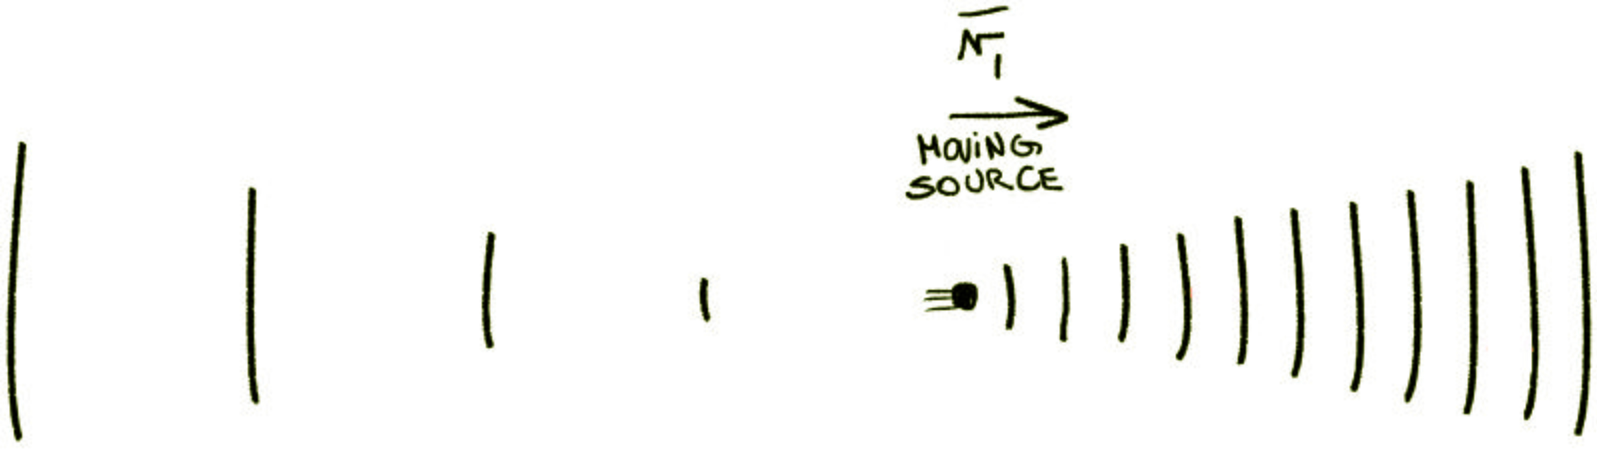
\includegraphics[height=1.2in]{images4/doppler3.jpg}
% \end{center}


%   \end{frame}

%%%%%%%%%%%%%%%%%%%%%%%%%%%%%%%%%%%%%%%%%%%%%%%%%%%%%%%%%%%%%%%


% \begin{frame}
% \frametitle{Doppler Effect}



% Source in motion $\rightarrow$ the wave travels at the velocity of sound in the air (its velocity is independent of the source velocity).




%   \begin{center}
%   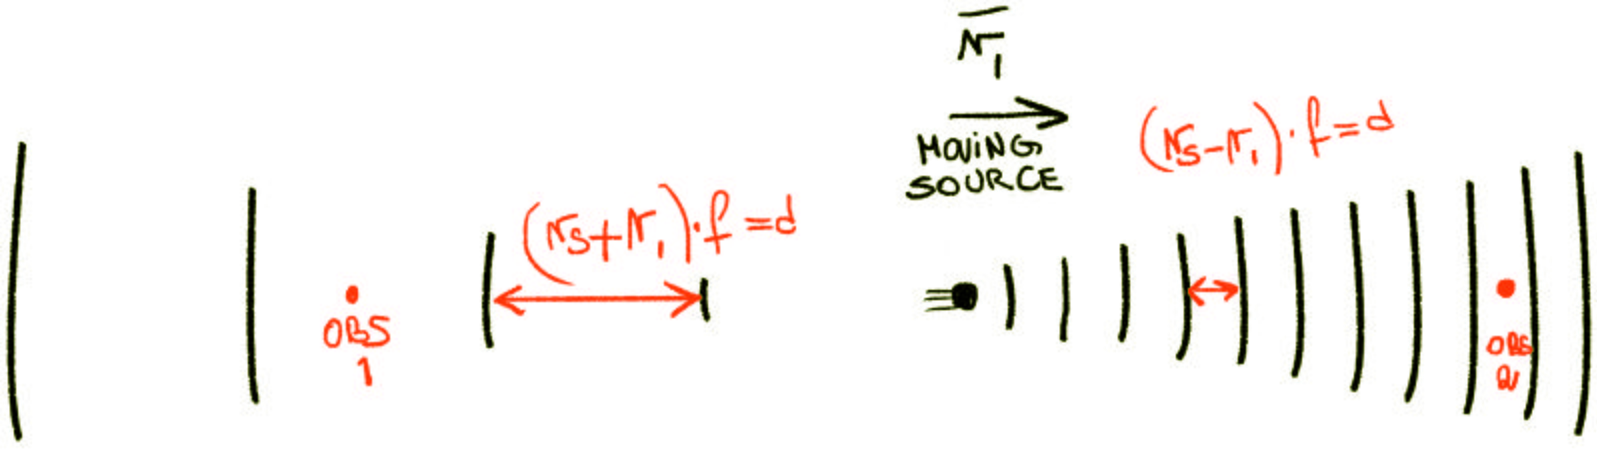
\includegraphics[height=1.2in]{images4/doppler4.jpg}
% \end{center}


%   \end{frame}



%%%%%%%%%%%%%%%%%%%%%%%%%%%%%%%%%%%%%%%%%%%%%%%%%%%%%%%%%%%%%%%

\begin{frame}
\frametitle{Doppler Effect}


The wavelength of a source traveling toward the observer is:

\begin{equation}
\lambda'=(v_{snd}-v_{src})T
\end{equation}


  \end{frame}
%%%%%%%%%%%%%%%%%%%%%%%%%%%%%%%%%%%%%%%%%%%%%%%%%%%%%%%%%%%%%%%

\begin{frame}
\frametitle{Doppler Effect}


Then, the wavelength of a source traveling toward the observer is:

\begin{equation}
\lambda'=(v_{snd}-v_{src})T=(v_{snd}-v_{src})\frac{\lambda}{v_{snd}}
\end{equation}


  \end{frame}
%%%%%%%%%%%%%%%%%%%%%%%%%%%%%%%%%%%%%%%%%%%%%%%%%%%%%%%%%%%%%%%

\begin{frame}
\frametitle{Doppler Effect}


Then, the wavelength of a source traveling toward the observer is:

\begin{equation}
\lambda'=(v_{snd}-v_{src})T=(v_{snd}-v_{src})\frac{\lambda}{v_{snd}}=\lambda(1-\frac{v_{src}}{v_{snd}})
\end{equation}

\pause

\vspace{5mm}

Where we consider that the source velocity is lower than the sound velocity. 
  \end{frame}

%%%%%%%%%%%%%%%%%%%%%%%%%%%%%%%%%%%%%%%%%%%%%%%%%%%%%%%%%%%%%%%

\begin{frame}
\frametitle{Doppler Effect}


Then, the shift in wavelength is,

\pause
\begin{equation}
\Delta \lambda=-\lambda \frac{v_{src}}{v_{snd}},
\end{equation}
\pause

proportional to the source velocity.

  \end{frame}
%%%%%%%%%%%%%%%%%%%%%%%%%%%%%%%%%%%%%%%%%%%%%%%%%%%%%%%%%%%%%%%

\begin{frame}
\frametitle{Doppler Effect}


The frequency perceived by the observer is,

\begin{equation}
f'=\frac{v_{snd}}{\lambda '}=\frac{v_{snd}}{\lambda(1-\frac{v_{src}}{v_{snd}})}
\end{equation}


  \end{frame}

%%%%%%%%%%%%%%%%%%%%%%%%%%%%%%%%%%%%%%%%%%%%%%%%%%%%%%%%%%%%%%%

\begin{frame}
\frametitle{Doppler Effect}


The frequency perceived by the observer is,

\begin{equation}
f'=\frac{f}{(1-\frac{v_{src}}{v_{snd}})}
\end{equation}


The denominator is less than 1, then the observed frequency is grater than the source frequency.

  \end{frame}






%%%%%%%%%%%%%%%%%%%%%%%%%%%%%%%%%%%%%%%%%%%%%%%%%%%%%%%%%%%%%%%

\begin{frame}
\frametitle{Doppler Effect}


If the source is moving away the observer,

\begin{equation}
\lambda'=(v_{snd}+v_{src})T=\lambda(1+\frac{v_{src}}{v_{snd}})
\end{equation}

\pause

The frequency is perceived by the observer is,

\pause

\begin{equation}
f'=\frac{f}{(1+\frac{v_{src}}{v_{snd}})}
\end{equation}

\pause

The observed frequency in this case is lower than the source frequency.


  \end{frame}





%%%%%%%%%%%%%%%%%%%%%%%%%%%%%%%%%%%%%%%%%%%%%%%%%%%%%%%%%%%%%%%

% \begin{frame}
% \frametitle{Doppler Effect}


% What happens if the source is at rest and the observer is moving toward the source?

% \pause

%   \begin{center}
%   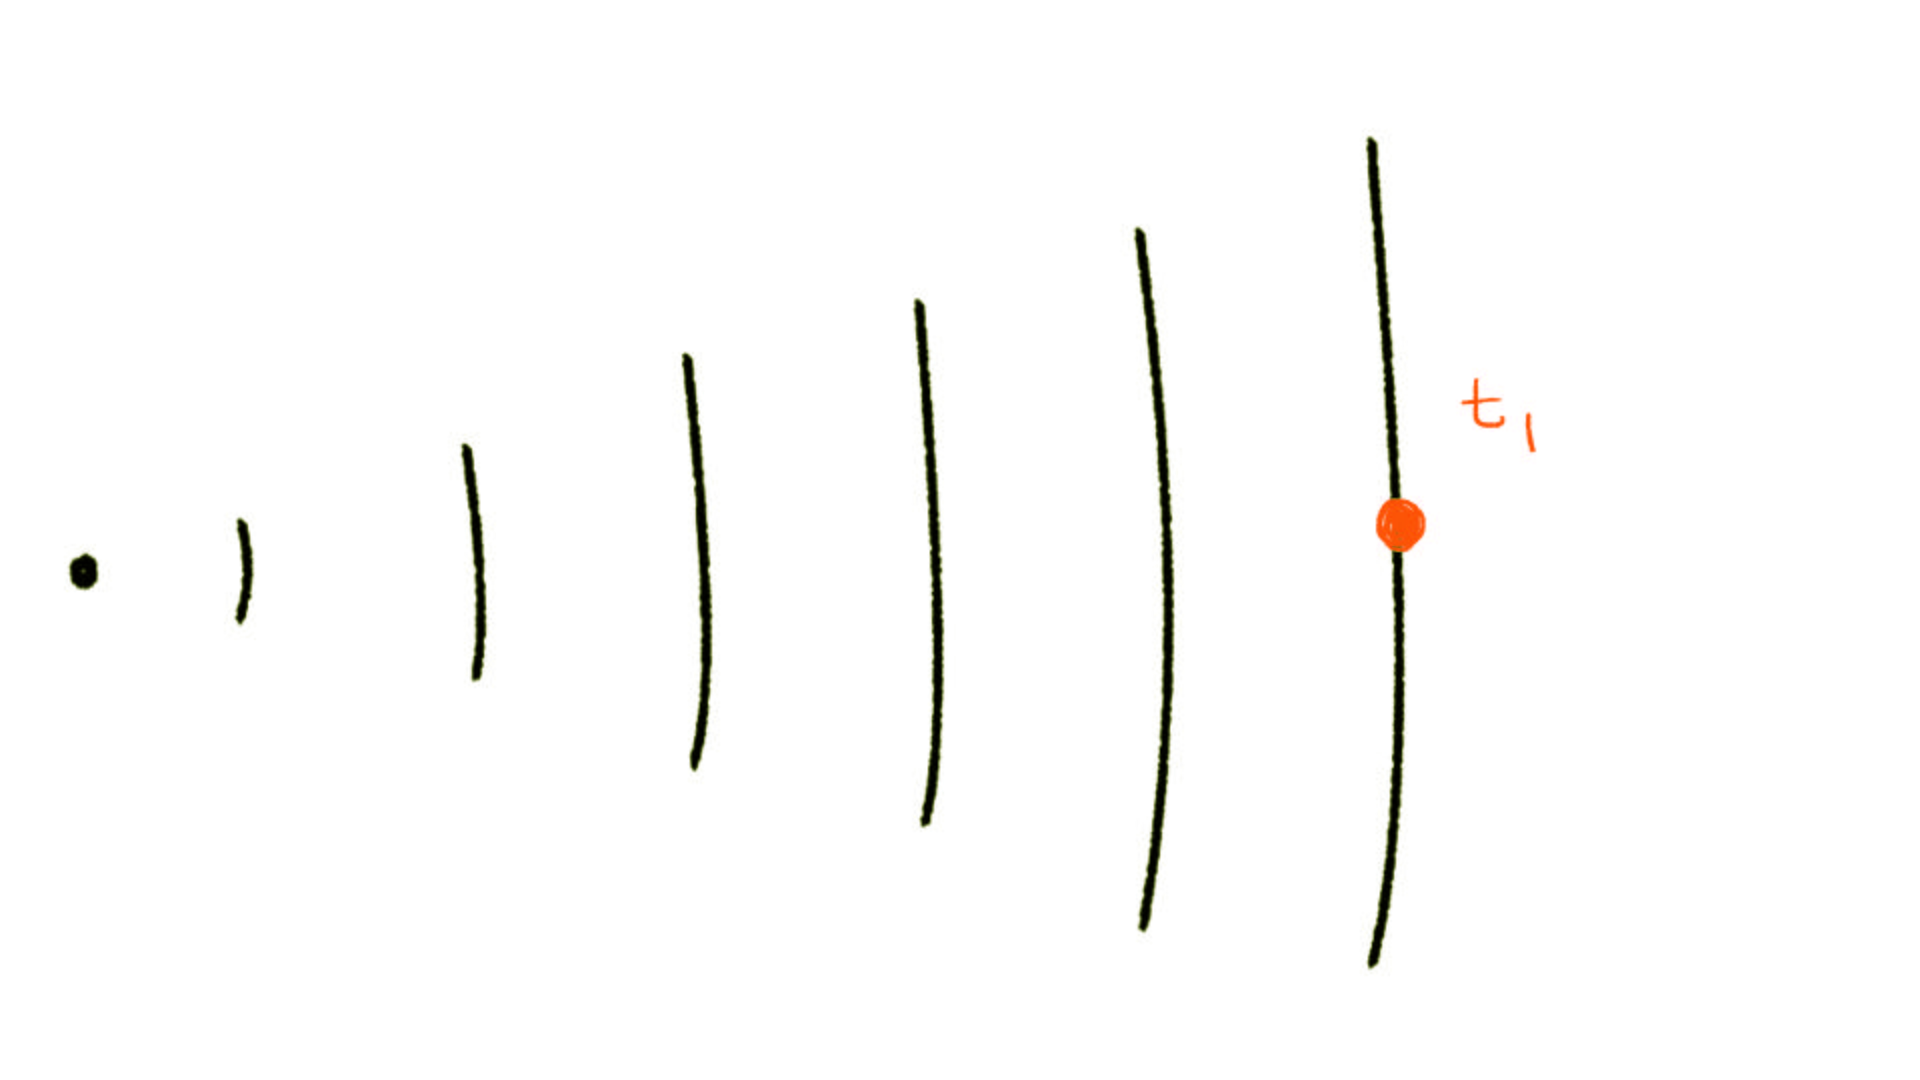
\includegraphics[height=1.2in]{images4/doppler5.jpg}
% \end{center}


%   \end{frame}



%%%%%%%%%%%%%%%%%%%%%%%%%%%%%%%%%%%%%%%%%%%%%%%%%%%%%%%%%%%%%%%

\begin{frame}
\frametitle{Doppler Effect}


What happens if the source is at rest and the observer is moving toward the source?



  \begin{center}
  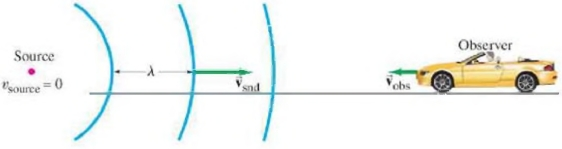
\includegraphics[height=1.0in]{images4/doppler6b.jpg}
\end{center}


  \end{frame}







%%%%%%%%%%%%%%%%%%%%%%%%%%%%%%%%%%%%%%%%%%%%%%%%%%%%%%%%%%%%%%%

\begin{frame}
\frametitle{Doppler Effect}


What is the frequency perceived by the observer that is moving toward the source?
\pause

\begin{equation}
f'=\frac{v_{snd}+v_{obs}}{\lambda}
\end{equation}



  \end{frame}










%%%%%%%%%%%%%%%%%%%%%%%%%%%%%%%%%%%%%%%%%%%%%%%%%%%%%%%%%%%%%%%

\begin{frame}
\frametitle{Doppler Effect}


What is the frequency perceived by the observer that is moving toward the source?

\begin{equation}
f'=\frac{v_{snd}+v_{obs}}{\lambda}=f\left(1+\frac{v_{obs}}{v_{sound}}\right)
\end{equation}



\pause
\vspace{5mm}

Quantitatively the change in frequency is different
than for the case of a moving source. 



  \end{frame}




%%%%%%%%%%%%%%%%%%%%%%%%%%%%%%%%%%%%%%%%%%%%%%%%%%%%%%%%%%%%%%%

\begin{frame}
\frametitle{Doppler Effect}



\begin{itemize}
\item Fixed source and a moving observer $\rightarrow$ $\lambda$ does change, but the velocity of the crest respect to the observer changes.\pause
\item Moving source and fixed observer  $\rightarrow$ $\lambda$ changes, but the velocity of the crest respect to the observer does not change. 
\end{itemize}

  \end{frame}




%%%%%%%%%%%%%%%%%%%%%%%%%%%%%%%%%%%%%%%%%%%%%%%%%%%%%%%%%%%%%%%

\begin{frame}
\frametitle{Doppler Effect}



If the observer is moving away from the source, the velocity of the crests respect to the observer is decreased, and the frequency is,
\pause

\vspace{5mm}

\begin{equation}
f'=\frac{v_{snd}-v_{obs}}{\lambda}=f\left(1-\frac{v_{obs}}{v_{sound}}\right)
\end{equation}

  \end{frame}



%%%%%%%%%%%%%%%%%%%%%%%%%%%%%%%%%%%%%%%%%%%%%%%%%%%%%%%%%%%%%%%

\begin{frame}
\frametitle{Doppler Effect}


When a sound wave is reflected from a moving obstacle, the frequency of the
reflected wave will, because of the Doppler effect, be different from that of
the incident wave.



  \end{frame}


%%%%%%%%%%%%%%%%%%%%%%%%%%%%%%%%%%%%%%%%%%%%%%%%%%%%%%%%%%%%%%%

\begin{frame}
\frametitle{Doppler Effect}

Example: Two Doppler shifts \pause

\vspace{3mm}

A $5000~Hz$ sound wave is emitted by a
stationary source. This sound wave reflects from an object moving $3.50~m/s$
toward the source. What is the frequency of the wave reflected by
the moving object as detected by a detector at rest near the source?                                                              




  \end{frame}



%%%%%%%%%%%%%%%%%%%%%%%%%%%%%%%%%%%%%%%%%%%%%%%%%%%%%%%%%%%%%%%

\begin{frame}
\frametitle{Doppler Effect}

Example: 

\vspace{3mm}

   \begin{columns}[c]
   \column{2in}  % slides are 3in high by 5in wide
  \begin{center}
  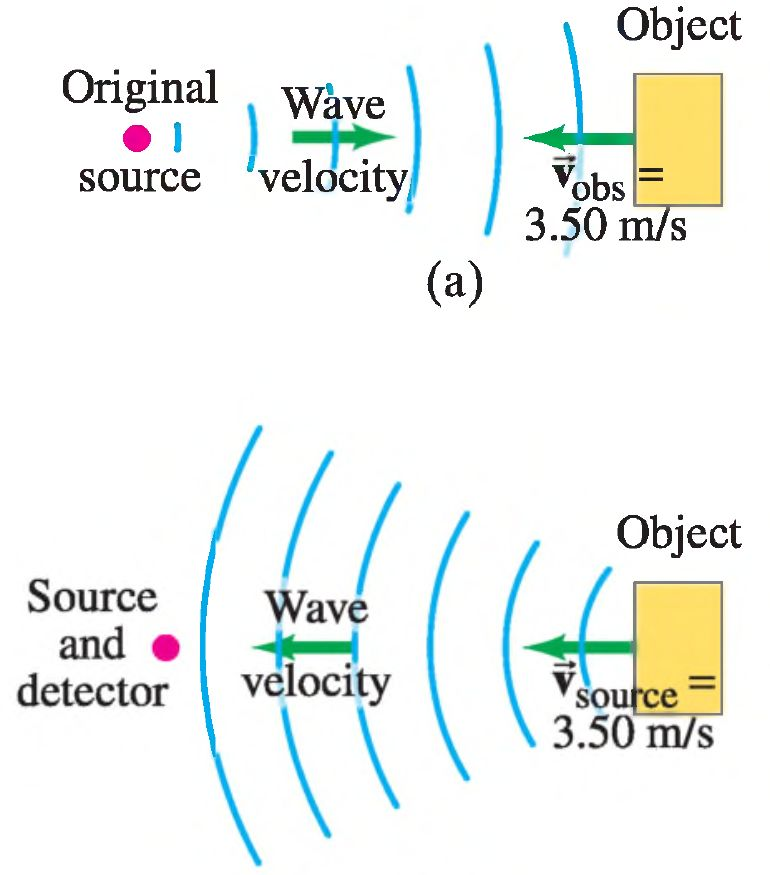
\includegraphics[height=2.in]{images4/doppler7.jpg}
\end{center}


  
   \column{2in}
\pause
The frequency detected by the moving object (obs) is:

\begin{equation*}
f'= f\left(1+\frac{v_{obs}}{v_{sound}}\right)
\end{equation*}




   \end{columns}




  \end{frame}

%%%%%%%%%%%%%%%%%%%%%%%%%%%%%%%%%%%%%%%%%%%%%%%%%%%%%%%%%%%%%%%

\begin{frame}
\frametitle{Doppler Effect}

Example: 

\vspace{3mm}

   \begin{columns}[c]
   \column{2in}  % slides are 3in high by 5in wide
  \begin{center}
  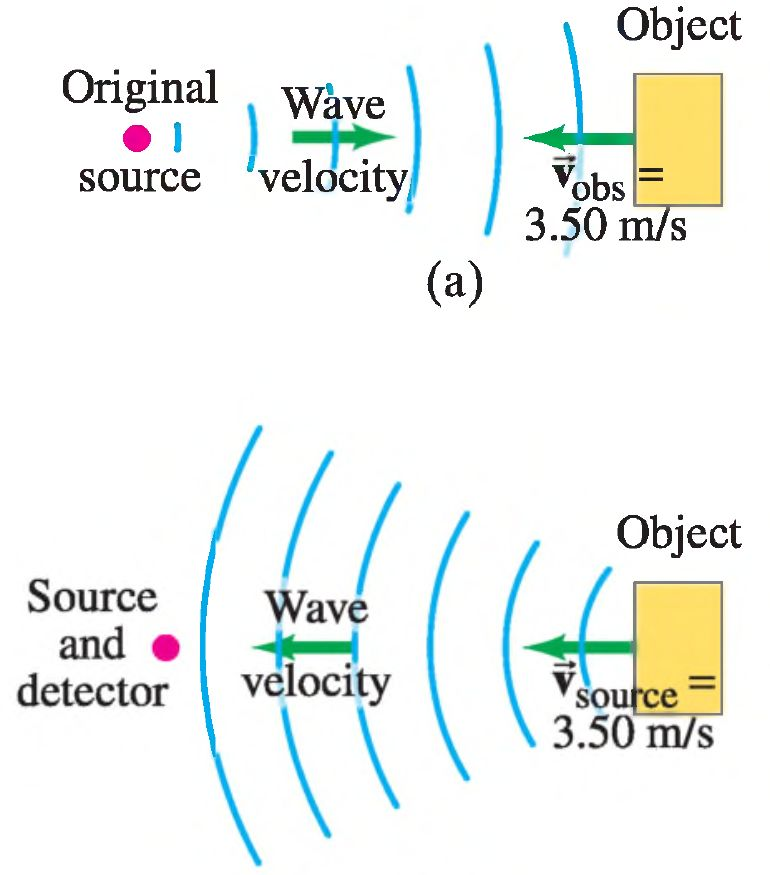
\includegraphics[height=2.in]{images4/doppler7.jpg}
\end{center}


  
   \column{2in}

   The frequency detected by the moving object (obs) is:

\begin{equation*}
f'= f\left(1+\frac{v_{obs}}{v_{sound}}\right)=5051~Hz
\end{equation*}




   \end{columns}




  \end{frame}


%%%%%%%%%%%%%%%%%%%%%%%%%%%%%%%%%%%%%%%%%%%%%%%%%%%%%%%%%%%%%%%

\begin{frame}
\frametitle{Doppler Effect}

Example: 

\vspace{3mm}

   \begin{columns}[c]
   \column{2in}  % slides are 3in high by 5in wide
  \begin{center}
  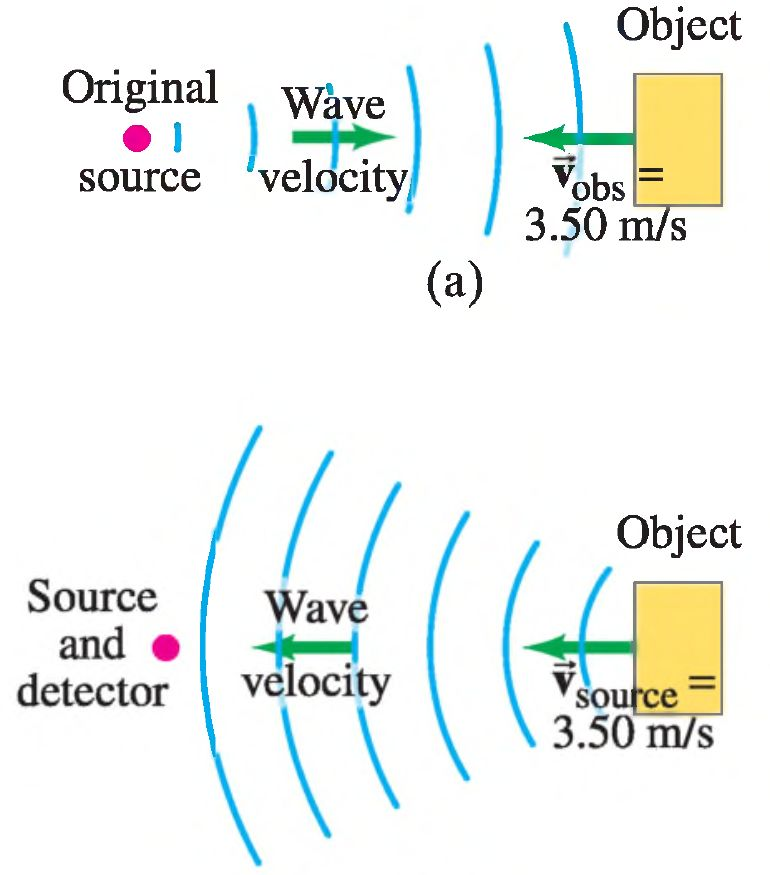
\includegraphics[height=2.in]{images4/doppler7.jpg}
\end{center}


  
   \column{2in}


The detected frequency is,

\begin{equation*}
f''=\frac{f'}{(1-\frac{v_{source}}{v_{snd}})}
\end{equation*}

   \end{columns}




  \end{frame}
%%%%%%%%%%%%%%%%%%%%%%%%%%%%%%%%%%%%%%%%%%%%%%%%%%%%%%%%%%%%%%%

\begin{frame}
\frametitle{Doppler Effect}

Example: 

\vspace{3mm}

   \begin{columns}[c]
   \column{2in}  % slides are 3in high by 5in wide
  \begin{center}
  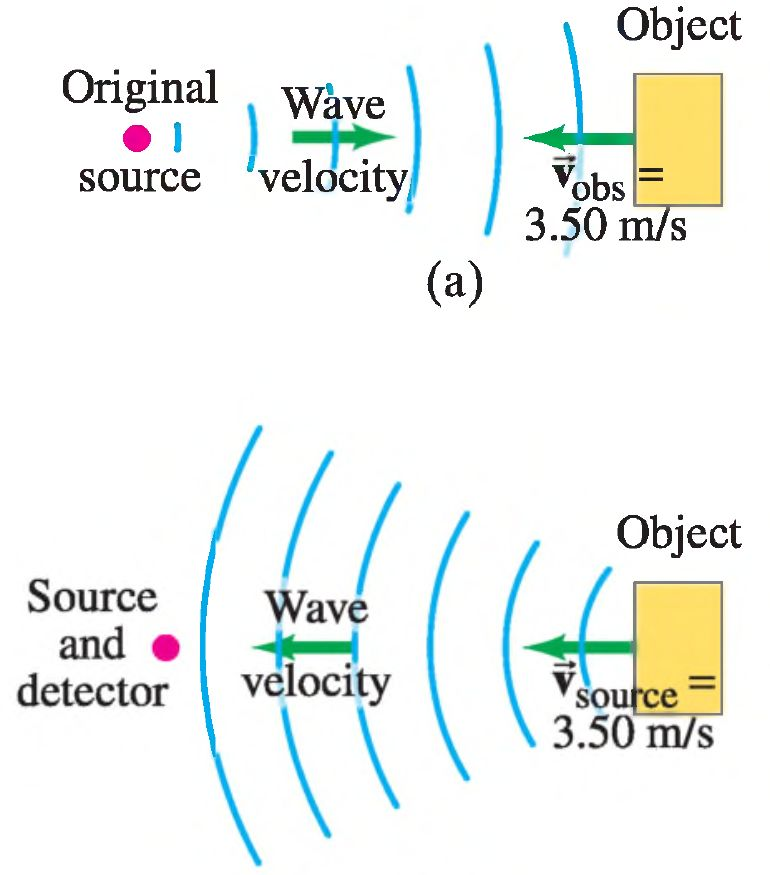
\includegraphics[height=2.in]{images4/doppler7.jpg}
\end{center}


  
   \column{2in}


The frequency emitted by the "new" source is,

\begin{equation*}
f''=\frac{f'}{(1-\frac{v_{source}}{v_{snd}})}=5103~HZ
\end{equation*}

   \end{columns}




  \end{frame}


%%%%%%%%%%%%%%%%%%%%%%%%%%%%%%%%%%%%%%%%%%%%%%%%%%%%%%%%%%%%%%%

\begin{frame}
\frametitle{Doppler Effect}

We can summarize both effects in a single equation:

\begin{equation*}
f'= f\left(1+\frac{v_{obs}}{v_{snd}}\right)
\end{equation*}


\begin{equation*}
f''=\frac{f'}{(1-\frac{v_{source}}{v_{snd}})}
\end{equation*}

\begin{equation}
f''= \frac{f}{(1-\frac{v_{source}}{v_{snd}})}\left(1+\frac{v_{obs}}{v_{snd}}\right)
\end{equation}


  \end{frame}


%%%%%%%%%%%%%%%%%%%%%%%%%%%%%%%%%%%%%%%%%%%%%%%%%%%%%%%%%%%%%%%

\begin{frame}
\frametitle{Doppler Effect}

Then, the frequency perceived by an observer when observer and source approach each other is,

\begin{equation}
f'=f \frac{v_{snd}+v_{obs}}{v_{snd}-v_{source}}
\end{equation}

\pause

And the frequency perceived  by an observer when observer and source move apart is,

\begin{equation}
f'=f \frac{v_{snd}-v_{obs}}{v_{snd}+v_{source}}
\end{equation}


  \end{frame}

%%%%%%%%%%%%%%%%%%%%%%%%%%%%%%%%%%%%%%%%%%%%%%%%%%%%%%%%%%%%%%%

\begin{frame}
\frametitle{Doppler Effect}

We can summarize all cases in a single equation:

\begin{equation}
f'=f \frac{v_{snd}\mp  v_{obs}}{v_{snd}\mp v_{source}}
\end{equation}

\pause
\vspace{5mm}
                                                       
The upper signs in numerator and denominator applies if
source and/or observer move toward each other; the lower signs applies if they are
moving apart.

  \end{frame}

%%%%%%%%%%%%%%%%%%%%%%%%%%%%%%%%%%%%%%%%%%%%%%%%%%%%%%%%%%%%%%%

\begin{frame}
\frametitle{Doppler Effect}

Application:
\pause

\vspace{3mm}


The incident wave and the reflected wave in the last example interfere with one another and beats are produced.
\pause

\begin{itemize}
\item measuring the beats frequency, we can obtain the value of the moving object.
\pause
\item  For example, ultrasonic waves
reflected from red blood cells can be used to determine the velocity of blood flow.
\pause
\item the technique can be used to detect the movement of the chest of a
young fetus and to monitor its heartbeat.
\end{itemize}


  \end{frame}

%%%%%%%%%%%%%%%%%%%%%%%%%%%%%%%%%%%%%%%%%%%%%%%%%%%%%%%%%%%%%%%

\begin{frame}
\frametitle{Doppler Effect}

What happens if the source travels at a velocity equal or higher the sound velocity?

\pause


  \begin{center}
  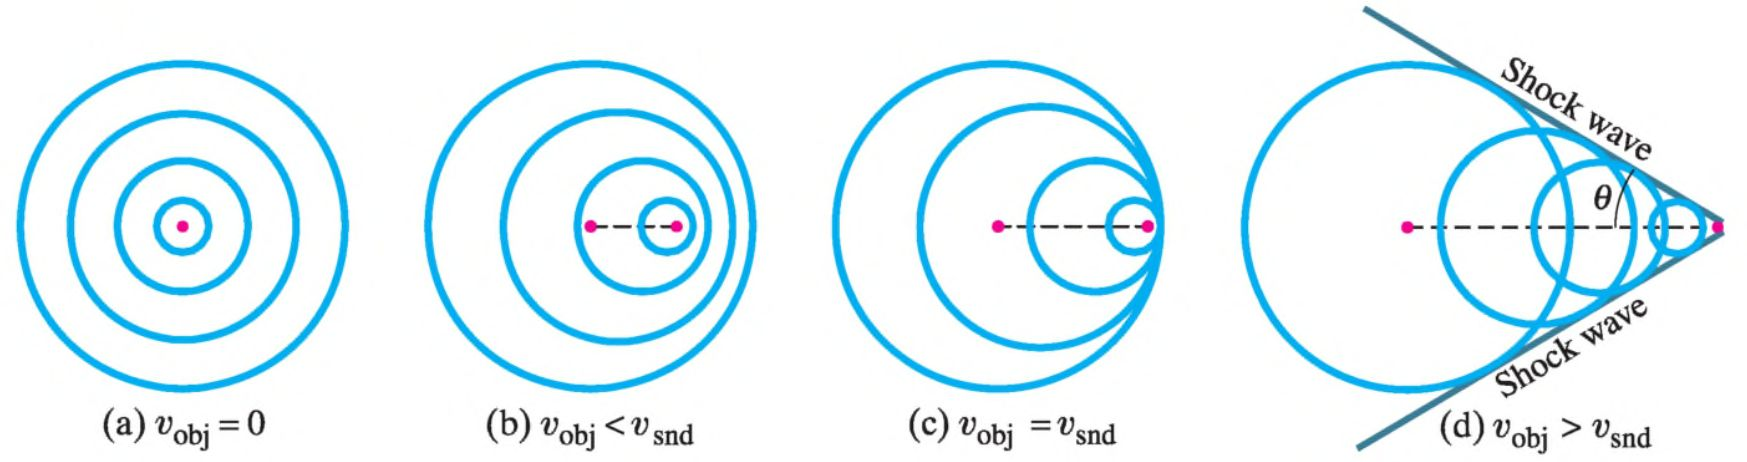
\includegraphics[height=1.2in]{images4/shock_wave.jpg}
\end{center}






  \end{frame}


%%%%%%%%%%%%%%%%%%%%%%%%%%%%%%%%%%%%%%%%%%%%%%%%%%%%%%%%%%%%%%%

\begin{frame}
\frametitle{Shock Waves}

\begin{itemize}
\item When $v_{obj}<v_{snd}$ the pitch changes as we have seen $\rightarrow$ Doppler effect (b).
\pause
\item When  $v_{obj}=v_{snd}$, the crest of the wave fronts overlap, creating a big crest or barrier called the "Sound Barrier" (c).
\pause
\item When $v_{obj}>v_{snd}$,the source has broken the sond barrier so it  is  “outrunning” the waves it produces. The crests of numerous wave fronts are overlapped producing a shock wave (d). 
\end{itemize}

\pause

\vspace{3mm}

A very clear explanation: \url{https://www.youtube.com/watch?v=If-yK7sQE8Q}  


  \end{frame}


%%%%%%%%%%%%%%%%%%%%%%%%%%%%%%%%%%%%%%%%%%%%%%%%%%%%%%%%%%%%%%%

\begin{frame}
\frametitle{Questions}

\begin{itemize}
\item Two tuning forks oscillate with the same amplitude, but one
has twice the frequency. Which (if either) produces the more
intense sound?
\pause
\item How will the air temperature in a room affect the pitch of
organ pipes?
\pause
\item Is there a Doppler shift if the source and observer move in
the same direction, with the same velocity? Explain.
\end{itemize}

  \end{frame}


%%%%%%%%%%%%%%%%%%%%%%%%%%%%%%%%%%%%%%%%%%%%%%%%%%%%%%%%%%%%%%%

\begin{frame}
\frametitle{Questions}

Consider the two waves shown in the figure. Each wave can
be thought of as a superposition of two sound waves with
slightly different frequencies. In which of
the waves, (a) or (b), are the two component frequencies
farther apart? Explain.

  \begin{center}
  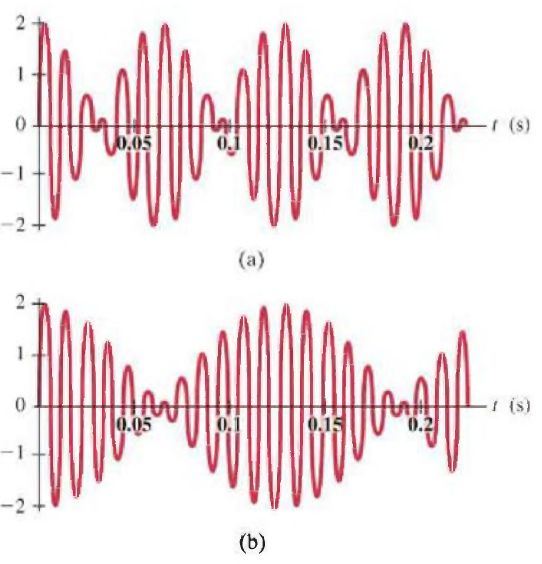
\includegraphics[height=1.5in]{images4/Q_ondas.jpg}
\end{center}


  \end{frame}


%%%%%%%%%%%%%%%%%%%%%%%%%%%%%%%%%%%%%%%%%%%%%%%%%%%%%%%%%%%%%%%

\begin{frame}
\frametitle{Questions}

The figure shows various positions of a child on a swing
moving toward a person on the ground who is blowing a
whistle. At which position, A through E, will the child hear
the highest frequency for the sound of the whistle? Explain
your reasoning.

  \begin{center}
  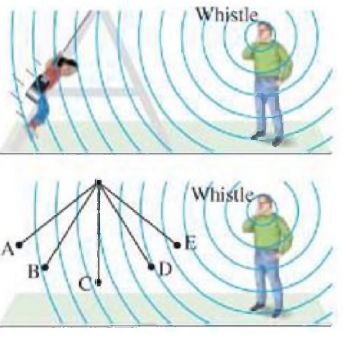
\includegraphics[height=1.5in]{images4/Q_ondas2.jpg}
\end{center}


  \end{frame}






%%%%%%%%%%%%%%%%%%%%%%%%%%%%%%%%%%%%%%%%%%%%%%%%%%%%%%%%%%%%%%%
 \end{document}
%%%%%%%%%%%%%%%%%%%%%%%%%%%%%%%%%%%%%%%%%%%%%%%%%%%%%%%%%%%%%%%